\subsection{Избыточное кодирование методом 4B/5B}

\item Исходное сообщение в двоичном коде:
\[
	\textbf{1100 0100 1110 0010 1100 0001 1100 0000}
\]

\item Логическое кодирование методом 4B/5B:
\[
	\begin{array}{l l}
		\text{1100} & \rightarrow \text{11010} \\
		\text{0100} & \rightarrow \text{01010} \\
		\text{1110} & \rightarrow \text{11100} \\
		\text{0010} & \rightarrow \text{10100} \\
		\text{1100} & \rightarrow \text{11010} \\
		\text{0001} & \rightarrow \text{01001} \\
		\text{1100} & \rightarrow \text{11010} \\
		\text{0000} & \rightarrow \text{11110} \\
	\end{array}
\]

\item Результирующее сообщение после 4B/5B кодирования (в двоичном виде):
\[
	\textbf{11010 01010 11100 10100 11010 01001 11010 11110}
\]

\item Результирующее сообщение после 4B/5B кодирования (в шестнадцатеричном виде):
\[
	\textbf{1A 2A 1C 14 1A 09 1A 1E}
\]

\item Длина нового собщения: 40 бит (5 байт)
\item Избыточность кодирования:
\[
	\text{Избыточность} = \frac{40 - 32}{32} \times 100 = 25\%
\]

Я бы мог применить логическое кодирование к методам кодирования, выбранным на втором этапе в качестве наилучших, но это бы совершенно не имело смысла, так как суть логического кодирования в том, чтобы обеспечить синхронизацию и устранить постоянную составляющую, в чём оба Манчестерских кодирования совершенно не нуждаются. Поэтому, я выберу NRZI как третий лучший метод для кодирования, в виду простоты, дешевизны и крайне узкого спектра, что обеспечит высокую скорость передачи сообщения, а при логическом кодировании будет обеспечена надёжная синхронизация и устранение постоянной составляющей.

\subsection{Применим для кодирования NRZI}
\begin{figure}[H]
	\centering
	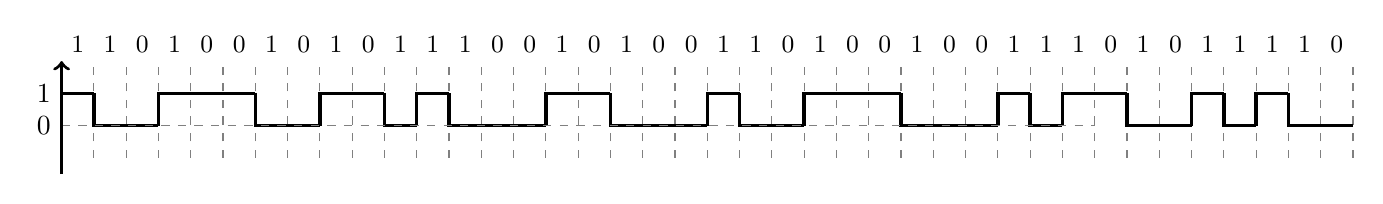
\begin{tikzpicture}[scale=0.41, very thick]
		\def\bits{1,1,0,1,0,0,1,0,1,0,1,1,1,0,0,1,0,1,0,0,1,1,0,1,0,0,1,0,0,1,1,1,0,1,0,1,1,1,1,0}

		\gdef\y{0}
		\foreach \b [count=\x from 0] in \bits {
			\draw[dashed, gray, thin] (\x+1,-1) -- (\x+1,2);
			\node at (\x+0.5, 2.5) {\small \b};
			\ifnum\b=1
				\ifnum\y=1
					\draw (\x,1) -- (\x,0) -- (\x+1,0);
					\xdef\y{0}
				\else
					\draw (\x,0) -- (\x,1) -- (\x+1,1);
					\xdef\y{1}
				\fi
			\else
				\draw (\x,\y) -- (\x+1,\y);
			\fi
		}

		\draw[dashed, gray, thin] (0,0) -- (32,0);
		\draw[->] (0,-1.5) -- (0,2);

		\node[left] at (0,0) {0};
		\node[left] at (0,1) {1};
	\end{tikzpicture}
	\caption{NRZI-кодирование избыточного сообщения}
\end{figure}

\begin{figure}[H]
	\centering
	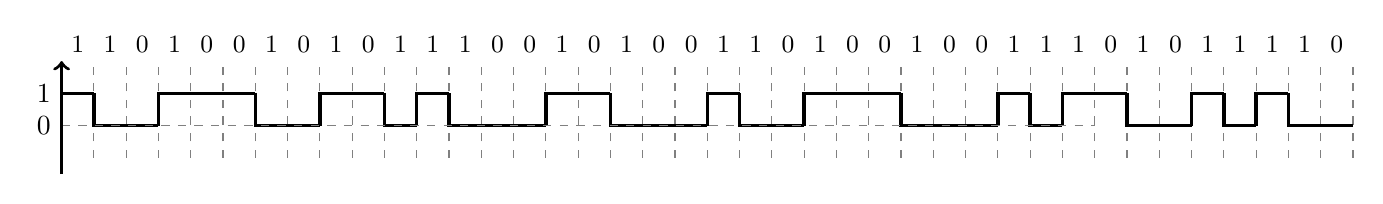
\begin{tikzpicture}[scale=0.41, very thick]
		\def\bits{1,1,0,1,0,0,1,0,1,0,1,1,1,0,0,1,0,1,0,0,1,1,0,1,0,0,1,0,0,1,1,1,0,1,0,1,1,1,1,0}

		\gdef\y{0}
		\foreach \b [count=\x from 0] in \bits {
			\draw[dashed, gray, thin] (\x+1,-1) -- (\x+1,2);
			\node at (\x+0.5, 2.5) {\small \b};
			\ifnum\b=1
				\ifnum\y=1
					\draw (\x,1) -- (\x,0) -- (\x+1,0);
					\xdef\y{0}
				\else
					\draw (\x,0) -- (\x,1) -- (\x+1,1);
					\xdef\y{1}
				\fi
			\else
				\draw (\x,\y) -- (\x+1,\y);
			\fi
		}

		\draw[dashed, gray, thin] (0,0) -- (32,0);
		\draw[->] (0,-1.5) -- (0,2);

		\node[left] at (0,0) {0};
		\node[left] at (0,1) {1};
	\end{tikzpicture}
	\caption{NRZI-кодирование избыточного сообщения}
\end{figure}

